%% =====================================================================
%%  L42i Paper Template  (built on the ACM acmart class)
%%  Lab for Interaction and Immersion, Georgia Tech School of Music
%%
%%  REUSING THIS FOR ANY COURSE
%%  Edit the COURSE INFO block a few lines down (course name, term,
%%  institution, ...). The course line on the paper updates itself.
%%
%%  HOW TO USE THIS TEMPLATE (for students)
%%  1. Replace the title, authors, and each \lipsum[...] with your own
%%     writing. The short comment above each section says what goes there.
%%  2. Anything in a comment (a line starting with %) is guidance for you
%%     and will NOT appear in the compiled PDF. Delete comments freely.
%%  3. Compile with pdfLaTeX. On Overleaf this is the default.
%%     Menu: Recompile.  Locally: run  latexmk -pdf L42i_paper_template.tex
%%  4. Keep acmart.cls, ACM-Reference-Format.bst, L42i_paper_template.bib,
%%     and the figures/ folder next to this file.
%% =====================================================================

%% =====================================================================
%%  PROVENANCE & LICENSE
%%  This file is a modified version of the ACM "acmart" sample
%%  sigconf.tex, by Boris Veytsman, adapted for course use. The acmart
%%  article class is distributed under the LaTeX Project Public License
%%  (LPPL) v1.3c or later; see https://ctan.org/pkg/acmart. Per the
%%  LPPL, this derivative has been renamed (L42i_paper_template.tex, not sigconf.tex)
%%  and is marked as modified.
%%
%%  This template is itself distributed under the LPPL v1.3c or later;
%%  see the LICENSE file. Modifications (c) 2026 Henrik von Coler / L42i.
%%
%%  Redistributed unmodified in this folder under their own terms:
%%    - acmart.cls .................. ACM acmart class, LPPL v1.3c
%%    - ACM-Reference-Format.bst .... public domain (per its own header)
%%  See NOTICE.txt for details.
%% =====================================================================

%% This is a course paper, so we turn OFF the ACM copyright/rights block
%% and reference-format requirements, and use the two-column conference
%% layout. You should not need to change this line.
\documentclass[sigconf, screen, nonacm]{acmart}

%% Optional: while drafting, you can switch to a single-column, wider-margin
%% layout with line numbers for easier feedback by using instead:
%%   \documentclass[manuscript, screen, nonacm, review]{acmart}

%% ---------------------------------------------------------------------
%% COURSE INFO  --  edit these lines to reuse the template for any class.
%% The number and instructor are optional: leave the braces empty to
%% hide them. This prints as a small footnote on page 1.
%% ---------------------------------------------------------------------
\newcommand{\coursename}{Technology Ensemble}
\newcommand{\coursenumber}{}                              % optional
\newcommand{\courseterm}{Fall}
\newcommand{\courseyear}{2026}
\newcommand{\courseinstitution}{Georgia Institute of Technology}
\newcommand{\coursedepartment}{School of Music}
\newcommand{\courseinstructor}{}                          % optional

%% Running header shown at the top of EVERY page (institution / school).
%% Leave the braces empty to turn the header off.
\newcommand{\pageheadertext}{Georgia Tech \textbullet\ School of Music}

%% These two lines suppress the leftover ACM reference/copyright
%% formatting (a class paper doesn't need it). Leave them alone.
\settopmatter{printacmref=false, printccs=false, printfolios=true}
\setcopyright{none}

%% Assembles the course line from the fields above. You don't need to
%% edit this --- optional fields appear only if you filled them in.
\newcommand{\courseline}{%
  Submitted for \emph{\coursename}%
  \ifdefempty{\coursenumber}{}{ (\coursenumber)}%
  , \courseterm~\courseyear, \courseinstitution, \coursedepartment.%
  \ifdefempty{\courseinstructor}{}{ Instructor: \courseinstructor.}%
}

%% BibTeX logo helper (leave this alone).
\AtBeginDocument{\providecommand\BibTeX{{Bib\TeX}}}

%% The body uses \lipsum[..] as placeholder ("Lorem ipsum") text so the
%% template reads the same for any class. Replace each \lipsum with your
%% own writing; once none are left, you can delete this package line.
\usepackage{lipsum}

%% ---------------------------------------------------------------------
%% CODE LISTINGS  --  used by the "Code" section below.
%% SuperCollider isn't a built-in listings language, so we define a small
%% keyword set here. For another course, change the keywords, or set
%% 'language' in \lstset to a built-in one (e.g. language=Python) and
%% delete this \lstdefinelanguage block.
%% ---------------------------------------------------------------------
\usepackage{listings}
\lstdefinelanguage{SuperCollider}{
  morekeywords={var,arg,SynthDef,Synth,SinOsc,EnvGen,Env,Out,perc,
                add,play,ar,kr,doneAction},
  sensitive=true,
  morecomment=[l]{//},
  morecomment=[s]{/*}{*/},
  morestring=[b]",
}
\lstset{
  language=SuperCollider,
  basicstyle=\ttfamily\small,
  keywordstyle=\bfseries,
  commentstyle=\color{gray},
  columns=fullflexible,
  keepspaces=true,
  breaklines=true,
  frame=single,
  framesep=6pt,
  xleftmargin=6pt,
}

%% Add any other packages you need below (example commented out):
%% \usepackage{tikz}       % for drawing diagrams

%% ---------------------------------------------------------------------
%% PAGE HEADER. Puts \pageheadertext (set in COURSE INFO) centered at the
%% top of every page, keeping acmart's title/author running heads and the
%% page number. To change the header, edit \pageheadertext above; to
%% remove it, set that to empty. (Assumes the default sigconf layout.)
%% This runs at \begin{document} so it applies after acmart sets its own
%% page styles.
%% ---------------------------------------------------------------------
\makeatletter
\AtBeginDocument{%
  \fancypagestyle{standardpagestyle}{%
    \fancyhf{}%
    \renewcommand{\headrulewidth}{\z@}%
    \renewcommand{\footrulewidth}{\z@}%
    \fancyfoot[C]{\if@ACM@printfolios\footnotesize\thepage\fi}%
    \fancyhead[L]{\ACM@linecountL\@headfootfont\shorttitle}%
    \fancyhead[R]{\@headfootfont\@shortauthors\ACM@linecountR}%
    \ifdefempty{\pageheadertext}{}{\fancyhead[C]{\@headfootfont\pageheadertext}}%
  }%
  \fancypagestyle{firstpagestyle}{%
    \fancyhf{}%
    \renewcommand{\headrulewidth}{\z@}%
    \renewcommand{\footrulewidth}{\z@}%
    \fancyfoot[C]{\if@ACM@printfolios\footnotesize\thepage\fi}%
    \ifdefempty{\pageheadertext}{}{\fancyhead[C]{\@headfootfont\pageheadertext}}%
  }%
  \pagestyle{standardpagestyle}%
}
\makeatother

\begin{document}

%% ---------------------------------------------------------------------
%% TITLE
%% Capitalize the title normally. If the title is long, put a short
%% version in the square brackets for the page header.
%% ---------------------------------------------------------------------
\title[Short Title]{The Title: A Template for Coursework}
%% This footnote stamps the paper with the course (COURSE INFO block
%% above). You don't need to edit it.
\titlenote{\courseline}

%% ---------------------------------------------------------------------
%% AUTHORS
%% This example shows a four-student group. Give each author their own
%% \affiliation block --- this is what produces ACM's side-by-side author
%% grid. Add or remove \author blocks to match your group. Authors at the
%% same school still each get a block (just repeat the same affiliation).
%% ---------------------------------------------------------------------
\author{Student One}
\email{sone@gatech.edu}
\affiliation{%
  \institution{Georgia Institute of Technology}
  \city{Atlanta}
  \state{Georgia}
  \country{USA}}

\author{Student Two}
\email{stwo@gatech.edu}
\affiliation{%
  \institution{Georgia Institute of Technology}
  \city{Atlanta}
  \state{Georgia}
  \country{USA}}

\author{Student Three}
\email{sthree@gatech.edu}
\affiliation{%
  \institution{Georgia Institute of Technology}
  \city{Atlanta}
  \state{Georgia}
  \country{USA}}

\author{Student Four}
\email{sfour@gatech.edu}
\affiliation{%
  \institution{Georgia Institute of Technology}
  \city{Atlanta}
  \state{Georgia}
  \country{USA}}

%% Short author list used in the page header. Update to match your authors.
\renewcommand{\shortauthors}{One, Two, Three, and Four}

%% ---------------------------------------------------------------------
%% ABSTRACT  --  a short paragraph: what you did, why, how, what you found.
%% Write it last, once the paper is done. (Placeholder text below.)
%% ---------------------------------------------------------------------
\begin{abstract}
  \lipsum[1]
\end{abstract}

%% ---------------------------------------------------------------------
%% KEYWORDS (optional --- delete if you prefer). A few comma-separated
%% terms describing the work.
%% ---------------------------------------------------------------------
\keywords{keyword one, keyword two, keyword three}

%% ---------------------------------------------------------------------
%% TEASER FIGURE (OPTIONAL). A wide image spanning both columns, shown
%% above the body. It is optional: to leave it out, delete this whole
%% block. To use it, replace figures/teaser.png with your own image.
%% ---------------------------------------------------------------------
\begin{teaserfigure}
  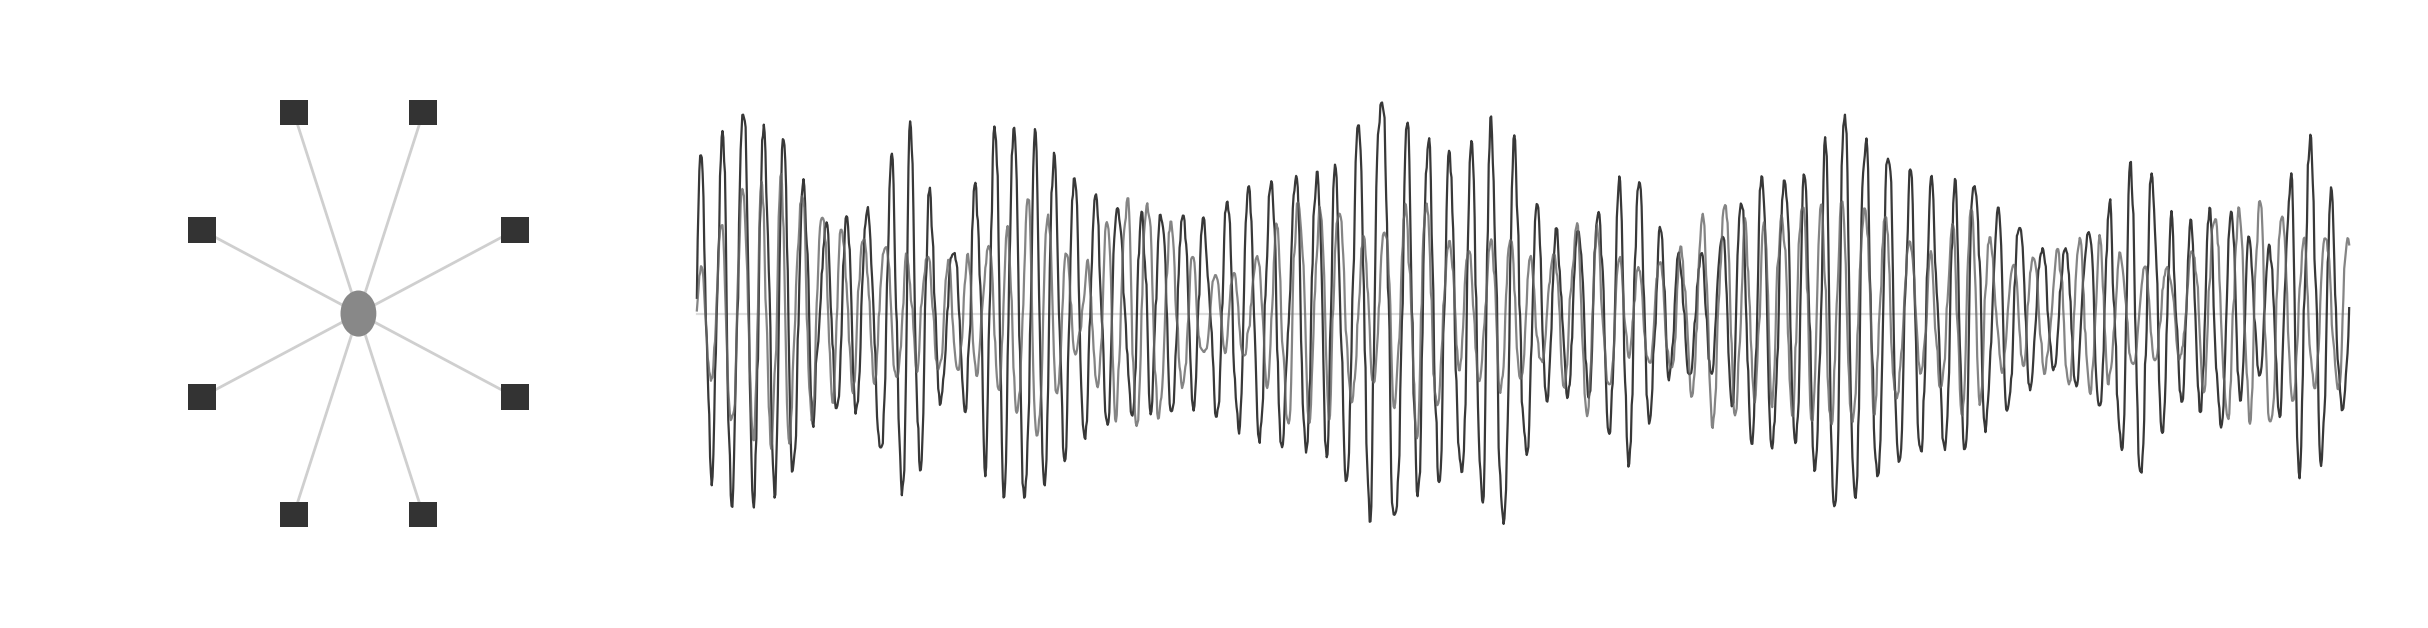
\includegraphics[width=\textwidth]{figures/teaser}
  \caption{Optional teaser image spanning both columns. Replace it with
    your own image, or delete this block entirely.}
  \Description{Describe the teaser image here for accessibility.}
\end{teaserfigure}

\maketitle

%% =====================================================================
%%  BODY
%%  The sections below are a suggested structure for a project paper.
%%  Rename, merge, split, or reorder them to fit YOUR project. Replace
%%  every \lipsum[..] with your own text; the comment over each section
%%  says what belongs there. The figure, equation, table, code, and
%%  citation are kept as working examples --- reuse their mechanics,
%%  replace their content.
%% =====================================================================

\section{Example Section: Citations}
%% Situate the work; cite what it builds on or reacts to.
\lipsum[3]
Cite sources inline --- one like this~\cite{puckette2007}, or several
like this~\cite{smalley1997spectromorphology, supercollider}. Entries live in the
\texttt{.bib} file, and the numbering is automatic.

\section{Example Section: Figures}
%% The design or method at a conceptual level. A diagram often helps ---
%% refer to it by its \label, as shown.
\lipsum[4]

A block diagram is often the clearest overview (Figure~\ref{fig:example}).

\begin{figure}[h]
  \centering
  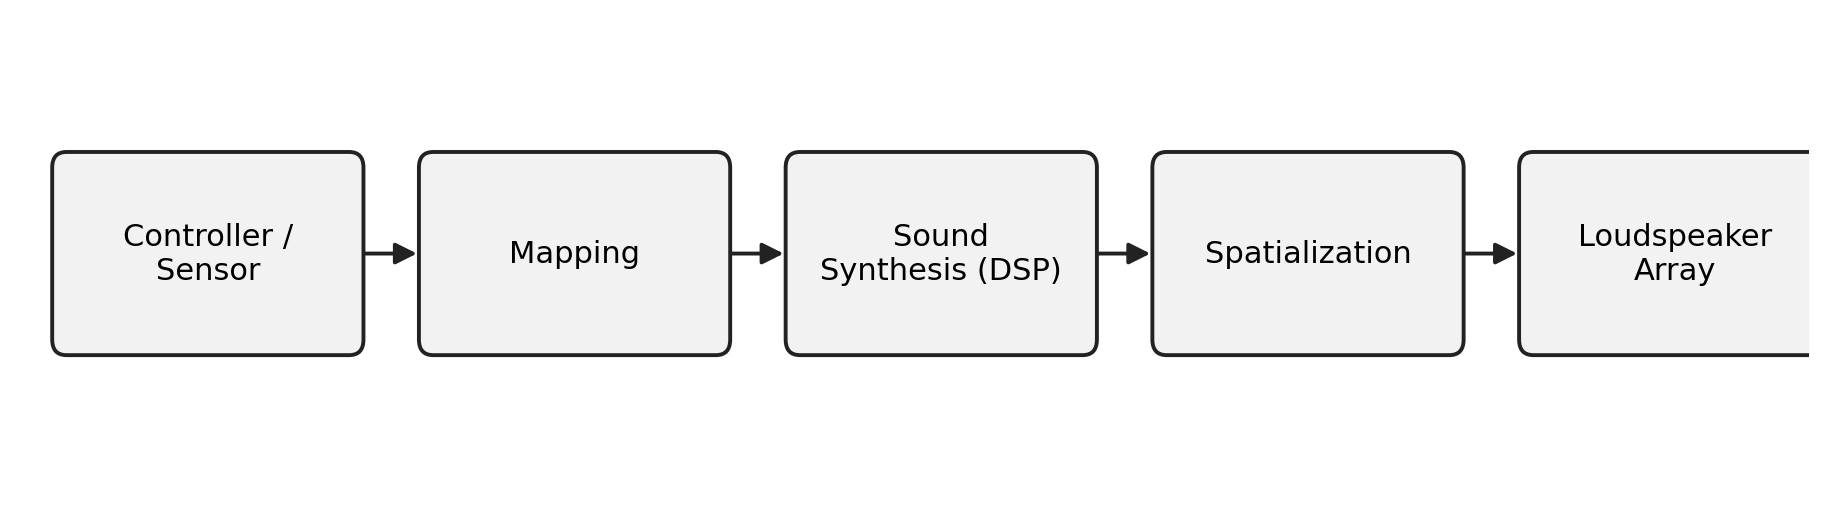
\includegraphics[width=\columnwidth]{figures/signal-flow}
  \caption{Example figure. Replace it with your own and update the
    caption and label.}
  \Description{Describe the figure here for accessibility.}
  \label{fig:example}
\end{figure}

\section{Example Section: Equations}
%% The concrete how: tools, materials, steps. Show key equations if they
%% matter --- number them and refer back by \label, as shown.
\lipsum[5]
Set and reference equations by number, as in Equation~\ref{eq:example}:
\begin{equation}
  y = a\,x + b .
  \label{eq:example}
\end{equation}


\section{Example Section: Code}
%% Show code when it helps. Use \lstinline for a short snippet inside a
%% sentence, and the lstlisting environment for a block you can caption
%% and reference. The listings setup (and language) is in the preamble.

Name code inline like \lstinline|SinOsc.ar(440)| when it belongs in a
sentence. For anything longer, set it as a listing you can caption and
refer to by label, as in Listing~\ref{lst:example}.

\begin{lstlisting}[caption={Example SuperCollider code.}, label={lst:example}]
// a simple synth: a sine tone with a percussive envelope
SynthDef(\ping, { arg freq = 440, amp = 0.2;
    var env = EnvGen.kr(Env.perc(0.01, 0.5), doneAction: 2);
    var sig = SinOsc.ar(freq) * env * amp;
    Out.ar(0, sig ! 2);
}).add;

// play one note
Synth(\ping, [\freq, 660]);
\end{lstlisting}

\lipsum[2]


\section{Example Section: Tables}
%% What happened: observations, measurements, outcomes. A table can
%% summarize structured results (Table~\ref{tab:example}).
\lipsum[6]

\begin{table}[h]
  \centering
  \caption{Example table --- replace the rows with your own.}
  \label{tab:example}
  \begin{tabular}{ll}
    \toprule
    Item & Value \\
    \midrule
    First item   & Value A \\
    Second item  & Value B \\
    Third item   & Value C \\
    \bottomrule
  \end{tabular}
\end{table}


%% ---------------------------------------------------------------------
%% ACKNOWLEDGMENTS (optional). Use this environment, not a \section.
%% ---------------------------------------------------------------------
% \begin{acks}
%   Thank collaborators and anyone who helped with the project here.
%   Delete this section if you don't need it.
% \end{acks}

%% ---------------------------------------------------------------------
%% REFERENCES
%% Add your sources to L42i_paper_template.bib and cite them with \cite{key}.
%% Only sources you actually cite will appear in the list.
%% ---------------------------------------------------------------------
\bibliographystyle{ACM-Reference-Format}
\bibliography{L42i_paper_template}

%% ---------------------------------------------------------------------
%% APPENDIX (optional). Uncomment to add. Appendix sections are lettered.
%% Good for long code listings, extra diagrams, or full parameter tables.
%% ---------------------------------------------------------------------
% \appendix
% \section{Additional Material}
% Put supplementary content here.

\end{document}
